\documentclass{standalone}
\usepackage{tikz}
\usepackage{circuitikz}

\begin{document}
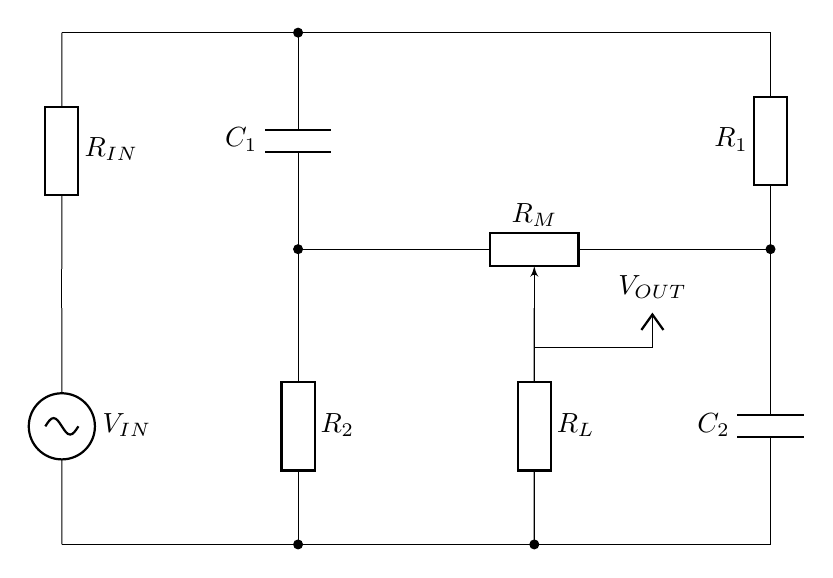
\begin{tikzpicture}
	\draw (1, 6.5) to[sinusoidal voltage source, l=$V_{IN}$] (1, 3.5);

	\draw (1, 10) to[european resistor, l=$R_{IN}$] (1, 7);
	\draw (10, 10) to[european resistor, l_=$R_1$] (10, 7.25);
	\draw (4, 6.5) to[european resistor, l=$R_2$] (4, 3.5);
	\draw (7, 6.5) to[european resistor, l=$R_L$] (7, 3.5);

	\draw (10, 7.25) to[european potentiometer, l_=$R_M$] (4, 7.25);

	\draw (4, 7.25) to[capacitor, l=$C_1$] (4, 10);
	\draw (10, 6.5) to[capacitor, l_=$C_2$] (10, 3.5);

	\draw (1, 10) -| (4, 10);
	\draw (1, 3.5) -- (10, 3.5);
	\draw (1, 6.5) -- (1, 7);
	\draw (4, 10) -- (10, 10);
	\draw (4, 6.5) -- (4, 7.25);
	\draw (7, 6) -- (8.5, 6);
	\draw (7, 6.69) -- (7, 6.5);
	\draw (10, 6.5) -- (10, 7.25);

	\node[vcc] at (8.5, 6) {$V_{OUT}$};
	\node[circ] at (10, 7.25) {};
	\node[circ] at (4, 10) {};
	\node[circ] at (4, 3.5) {};
	\node[circ] at (4, 7.25) {};
	\node[circ] at (7, 3.5) {};

\end{tikzpicture}
\end{document}